\documentclass[a4paper]{scrreprt}
\usepackage[german]{babel}
\usepackage[utf8]{inputenc}
\usepackage{graphicx}
\usepackage{hyperref}
\usepackage{pdflscape}
\usepackage{wrapfig}
\usepackage{adjustbox}
\usepackage{bbding}
\usepackage{subfiles}
\hypersetup{
    colorlinks,
    citecolor=black,
    filecolor=black,
    linkcolor=black,
    urlcolor=black
}


\begin{document}
\title{Qualitätssicherungsdokument}
\author{Hanselmann, Hecht, Klein, Schnell, Stapelbroek, Wohnig}
\date{\today\\v0.4}
\maketitle 
\tableofcontents	

\chapter{Einleitung}


\chapter{Codereviews}

\section{Planung}
Wir haben die Qualitätssicherungsphase mit Codereviews angefangen.
Hierfür wurde unsere Gruppe in Gruppen zu je zwei Leuten unterteilt, wobei
darauf Wert gelegt wird, dass diese, die sich gegenseitig ihren Code erklären
müssen, möglichst wenig über den Code des anderen wissen. Wir haben hiermit
angefangen, um möglichst schnell die gröbsten Fehler im Code zu finden, sodass
wir uns im weiteren Verlauf des Qualitätssicherung auf versteckter liegende konzentrieren
konnten. Ein weiterer wichtiger Aspekt dieser Codereviwes war, den Code zu
refactorn, um die Lesbarkeit, Wartbarkeit und spätere Testbarkeit zu erhöhen.

\section{Ergebnis}
Das Ergebnis der Codereviews ist nicht ganz eindeutig. Während sie manchen
Personen geholfen haben Fehler zu finden, die beim späteren Testen
wahrscheinlich nicht entdeckt worden wären, und den Code an sich etwas robuster
zu machen, haben andere eigentlich nur ein paar Style Fehler gefunden, und
angegeben, dass ihnen die Codereviews eigentlich nicht geholfen hätten. Dies
kann aber auch daran gelegen haben, dass die Leute zu schnell über den Code
gegangen sind, und die andere Person nicht tiefgründig genug gehende Fragen
gestellt hat.

\chapter{Unit-Tests}

\section{Planung}
Neben den Codereviews haben wir anfangs parallel (zum
Beispiel weil ein Gruppenmitglied einer Zweiergruppe keine Zeit hat und sein
Partner etwas zu tun braucht) und später auch
verstärkt darauf hinarbeiten Testfälle für den Code zu schreiben.
Zum einen werden wir alle Testfälle, welche im Pflichtenheft genannt wurden,
implementieren. Sollte der Testfall GUI Bezug haben oder an sich nicht mit JUnit
realisieren lassen wird er dann von Hand ausgefürt. Dabei ist es jedoch wichtig alle Schritte genau zu
dokumentieren, damit der Test, im Falle einer Änderung, auch später noch
reproduzierbar ist.

\section{Übersicht über gefundene Fehler}
Dank der Unit-Tests und dem Testen von Hand konnten in dieser Phase  viele
Fehler gefunden werden, sodass wir hier eine Übersicht über einige geben werde:

\begin{itemize}
  \item Es gab einen Fehler in der Codegenerierung, sodass zum Beispiel Voting
  Arrays, die gleich sein sollten, unterschiedlich waren.
  \item In manchen Fälle ließ sich die Analyse nicht starten.
  \item Ein paar Nullpointer Exceptions.
  \item Die Ausgabe von CBMC konnte nicht immer richtig geparsed werden.
  \item Ein Fehler in der Codegenerierung, wenn man "`EXISTSONE"' verwendet.
  \item Fehler bei der Präferenz Wahl, bei der Wähler Kandidaten die selbe
  Position geben konnten.
\end{itemize}


\section{Testüberdeckung}
Zur Bewertung unserer Tests setzten wir als Metrik auf die
"`Instruktionsüberdeckung"', da sich diese am leichtesten messen lässt, und für
so ein komplexes Programm gut anzeigt, welche Bereiche noch weiterer Tests
bedürfen.
Weiterhin wird aber auch darauf geachtet, dass in den Methoden der einzelnen Klassen eine möglichst hohe
Pfadüberdeckung gegeben ist. Da die Metrik-Werkzeuge, welche wir verwenden zwar
nicht überdeckte Pfade anzeigen, daraus aber keine Ausdrucksvolle Metrik bauen
können, fließt sie nicht in die Metrik an sich mit ein, auch wenn darauf
geachtet wurde.
\newline
Momentan erreiche wir eine Testabdeckung von ca 77 \% (Stand 15.3.17 am Abend).
Für das fertige Dokument kommt hier ein Graph hin, in dem man die Testabdeckung
im Laufe der Zei (mindestens zu jedem milestone) erkennen kann.

\chapter{Performance und Verbrauch:}
Über die Phase haben wir unser Programm stetig in einem Profiler betrachtet, um
schnell reagieren zu können, sollte eine Änderung in dieser Phase die
Lauffähigkeit unseres Programmes stärker als Erwartet beeinflussen.
\newline
Die war jedoch nicht der Fall, sodass der Resoucenverbraucht vor und nach der
Qualitätssicherungsphase relativ konstant geblieben ist.
\newline
Wie man in \ref{fig1} und \ref{fig2} erkennen kann, ist der Verlauf des
Speicherverbrauches so gut wie identisch mit ca 30MB, bevor der "`garbage
collector"' es wieder auf ca 10 MB herunterbringt. Anscheinend haben viele
unserer Objekte nur eine kurze Lebensdauer, woraus sich auch schließen ließe,
dass unser Programm im "`Leerlauf"' einen insignifikanten Speicherverbrauch hat,
der Computersysteme von heute vor keine große Aufgabe stellen sollte.
\newline
Vergleicht man nun \ref{fig3} mit \ref{fig4} sieht man, dass sich die
Unterschiede der Versionen, während eine Eigenschaft überprüft wird, schon
stärker unterscheiden. Während der Arbeitsspeicherverbrauch zwar noch relativ
ähnlich zwischen den beiden Versionen ist, sieht man, dass die Auslastung des
Prozessors schon deutliche Unterschiede aufweist, welche jedoch vor allem darauf
zurückzuführen sind, dass nicht die exakt gleichen Wahlverfahren verglichen
wurden, da sich im Laufe der Qualitätssicherungsphase etwas am System zum
Speichern der Wahlverfahren geändert hatte.
\newline
Der Grund, aus dem der Resourcenverbrauch bei der Überprüfung so viel höher
liegt, ist, dass in dieser Phase zum einen der Code, welcher an CBMC gesendet
werden muss, für jede Eigenschaft einzeln erzeugt wird, und auch mehrere Threads
konstant die Ausgabe von CBMC auffangen müssen.
Ist die Überprüfung jedoch abgeschlossen normalisiert sich der
Resourcenverbrauch wieder relativ schnell.

\newpage
\begin{figure}[ht]
	\centering
  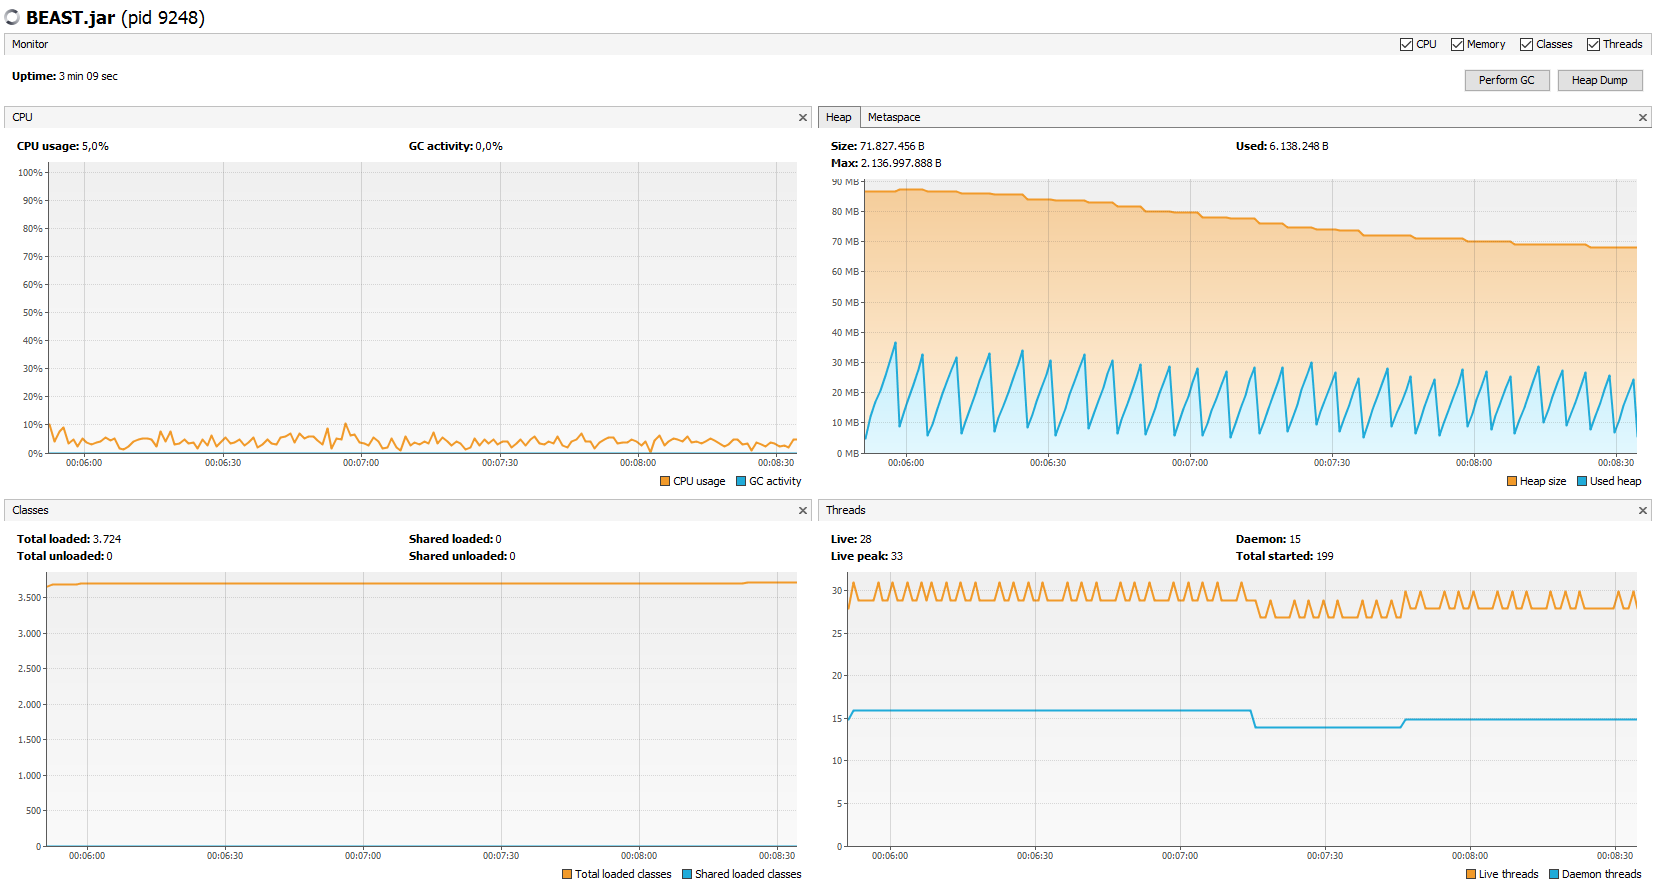
\includegraphics[width=1.0\textwidth,
  height=0.40\textwidth]{images/OLD_NO.png} \caption{Dies ist der
  Resoucenverbrauch des Programmes, während es auf eine Eingabe vom Nutzer wartet und momentan keine Verifikation durchführt}
	\label{fig1}
\end{figure}

\vspace{4cm}

\begin{figure}[ht]
	\centering
  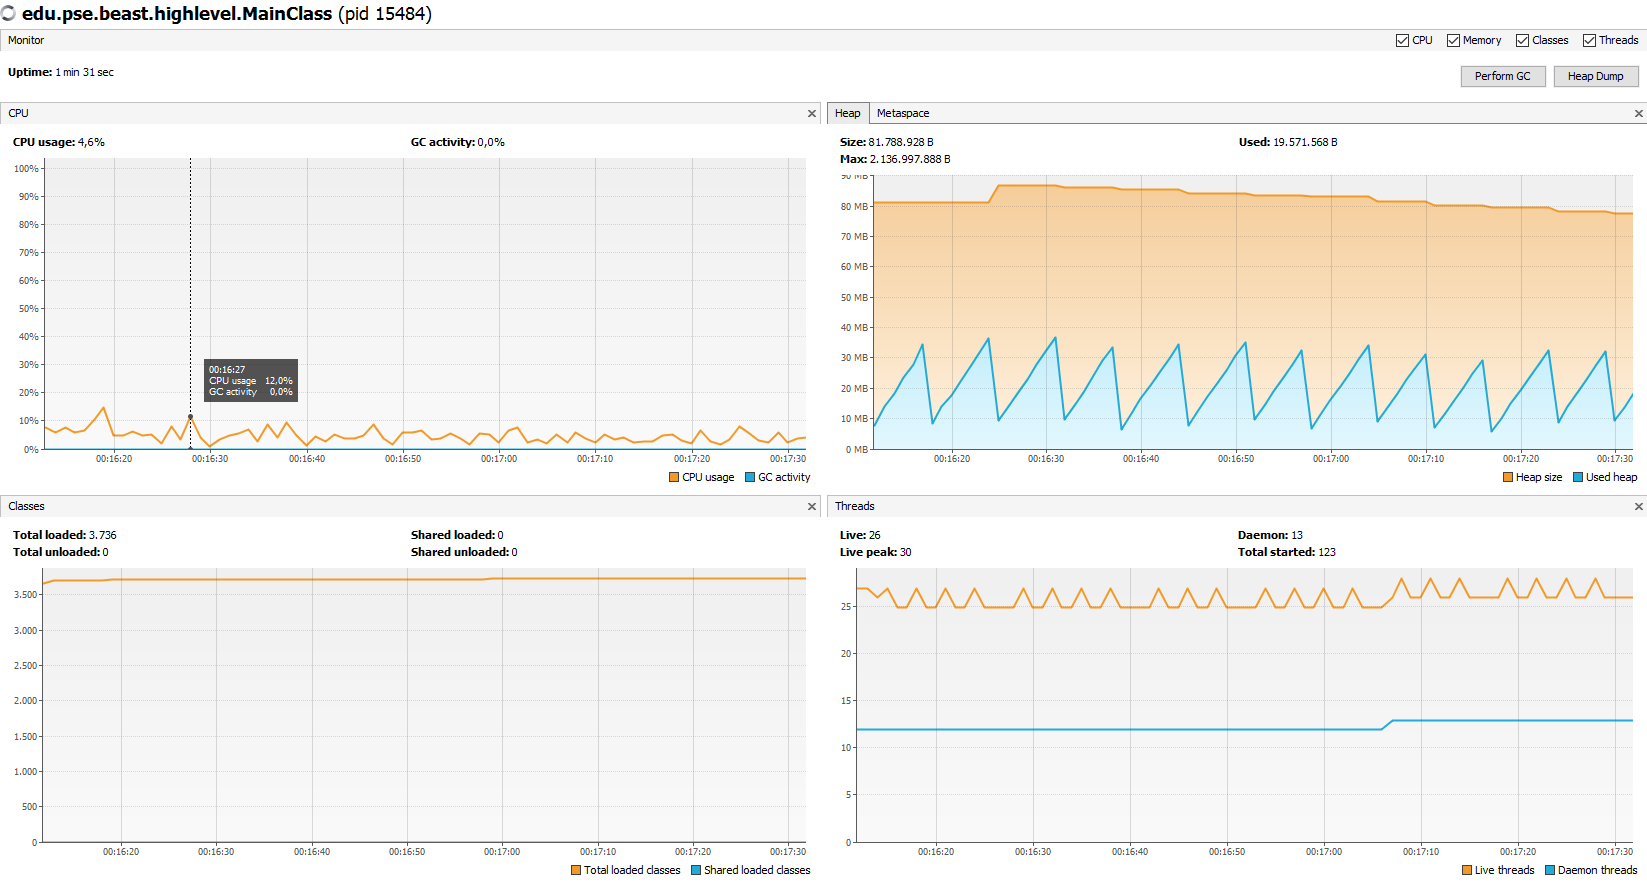
\includegraphics[width=1.0\textwidth,
  height=0.40\textwidth]{images/NEW_NO.png} \caption{Der Resourcenverbrauch der
  momentanten Version des Programmes, während keine Überprüfung durchgeführt wird}
	\label{fig2}
\end{figure}


\newpage

\begin{figure}[ht]
	\centering
  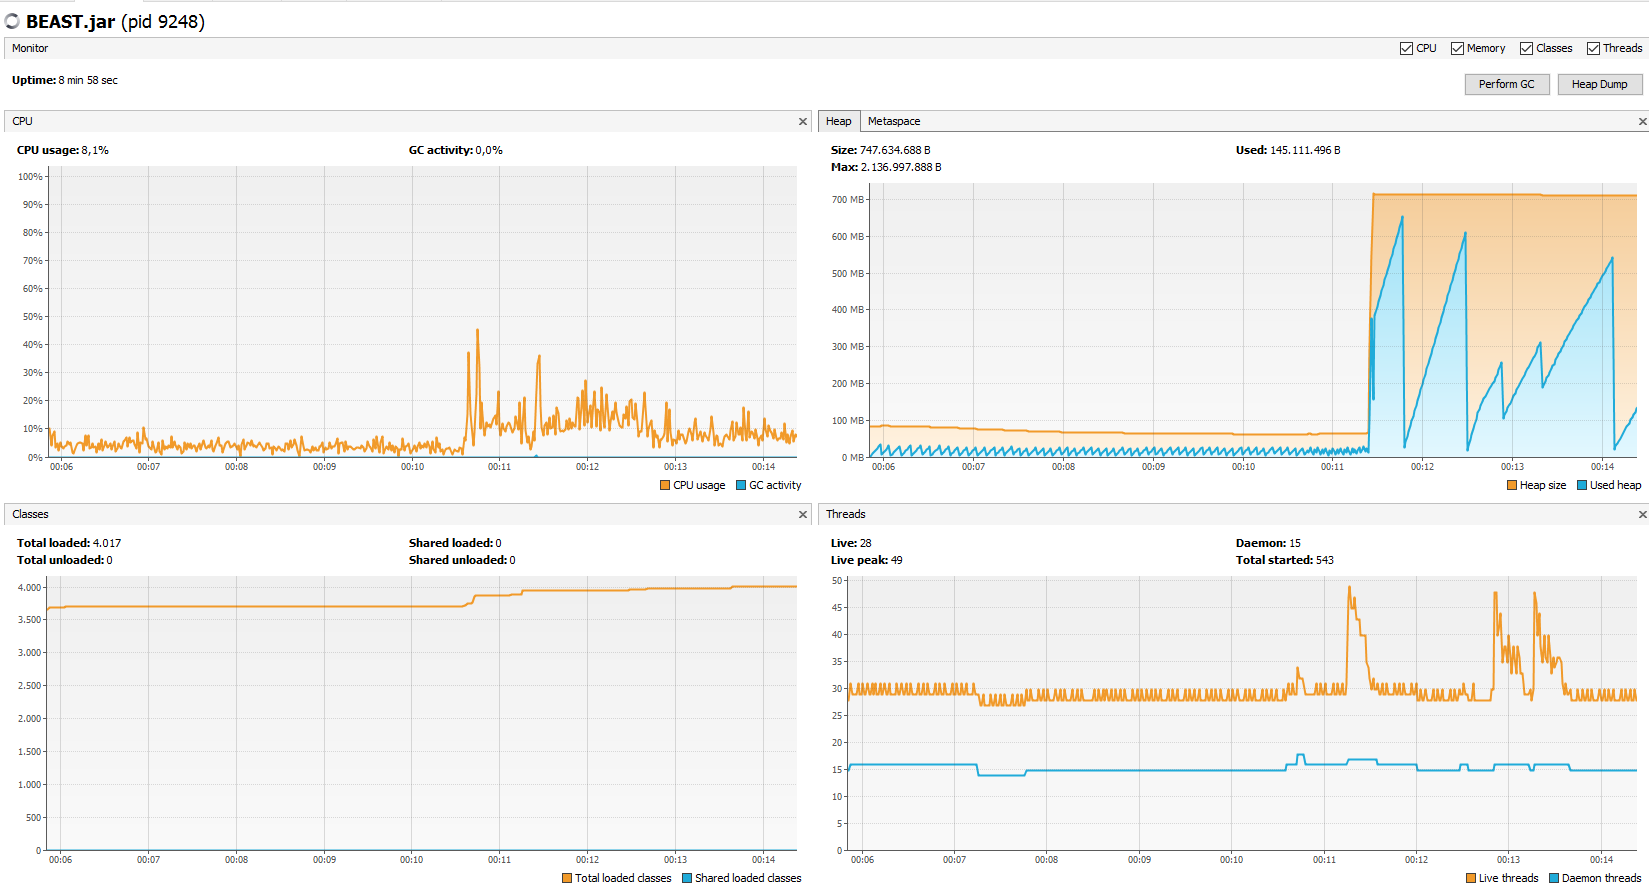
\includegraphics[width=1.0\textwidth,
  height=0.4\textwidth]{images/OLD_YES.png} \caption{Der Resourcenverbrauch
 der originalen Version von BEAST, während Eigenschaften überprüft werden}
	\label{fig3}
\end{figure}

\vspace{4cm}

\begin{figure}[ht]
	\centering
  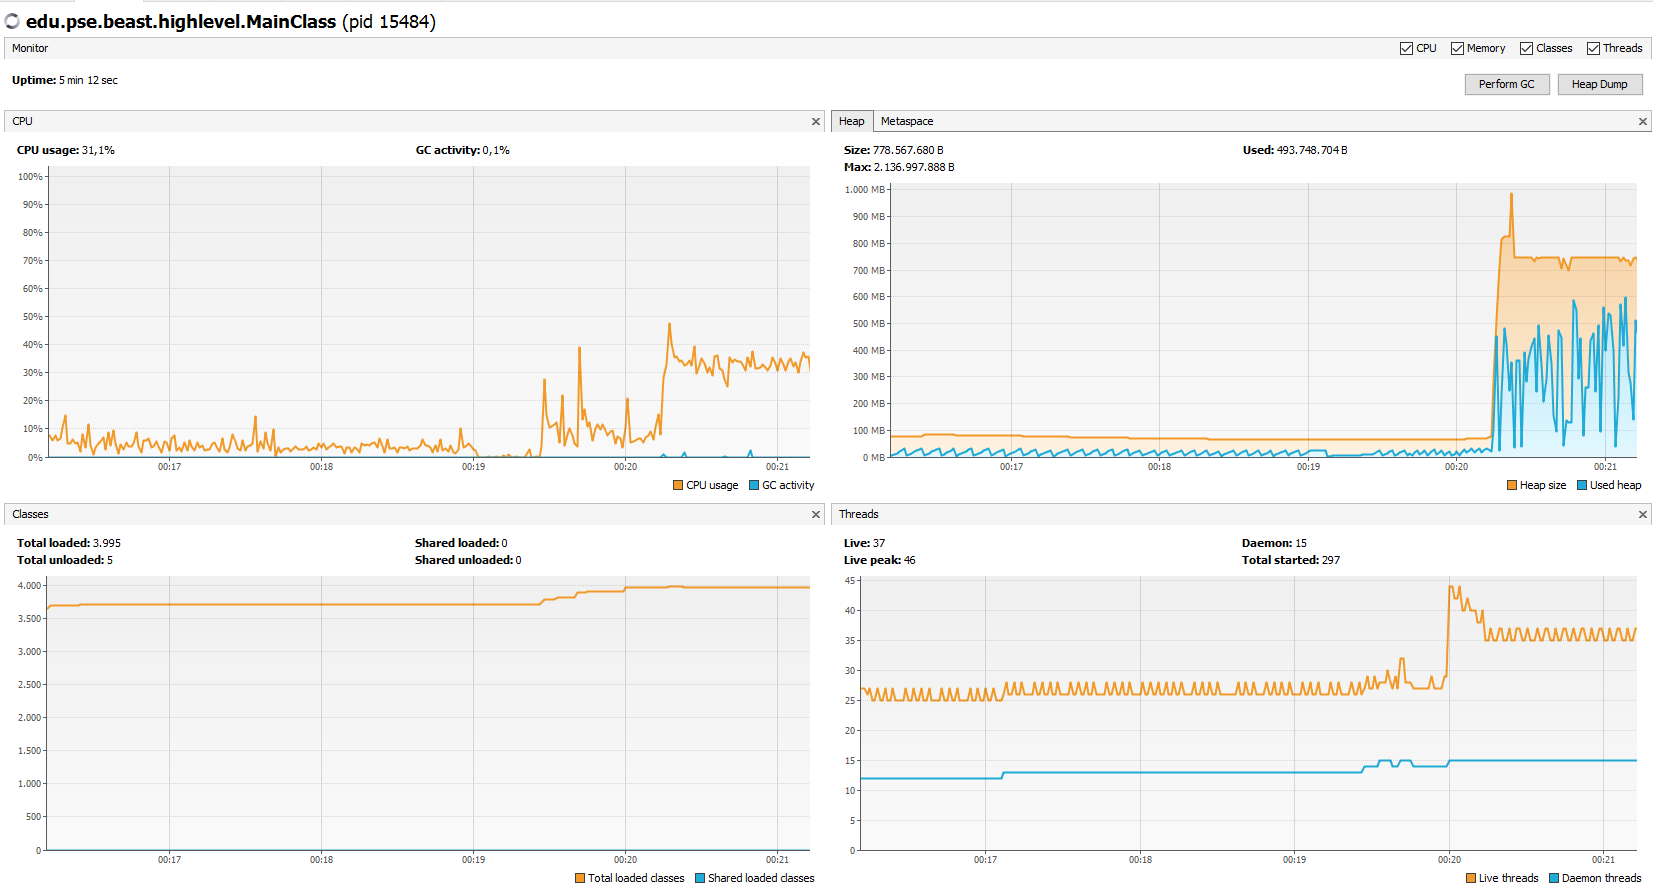
\includegraphics[width=1.0\textwidth,
  height=0.40\textwidth]{images/NEW_YES.png} \caption{Der Resourcenverbrauch der
  momentanten Version des Programmes, während Eigenschaften überprüft werden}
	\label{fig4}
\end{figure}

\newpage
Betrachtet man die Verteilung der neusten BEAST Version während einer
Analyse (siehe \ref{fig5}) fällt auf, dass die Methoden, welche die meiste
Prozessorzeit in Anspruch nehmen, die sind, die dafür sorgen, dass das Programm
so angenehmt für wie möglich läuft. Würde man zum Beispiel die konstante
Überprüfung auf Fehler weniger häuftig ausführen, so müsste der Nutzer länger auf eine
Rückmeldung warten, was er noch ändern müsste. Ähnlich verhält es sich zu den
"`ThreadedBufferedReader"' Instanzen, die auch noch einen großen Anteil an der
Prozessorzeit haben. Dies liegt daran, dass sie die gesamte Kommunikation zu
außerhalb laufenden Prozessen übernehmen, und deshalb die gesamte Zeit ohne
Unterbrechung laufen müssen, solange der Prozess, den sie Überwachen, auch noch
läuft.

\begin{figure}[ht]
	\centering
  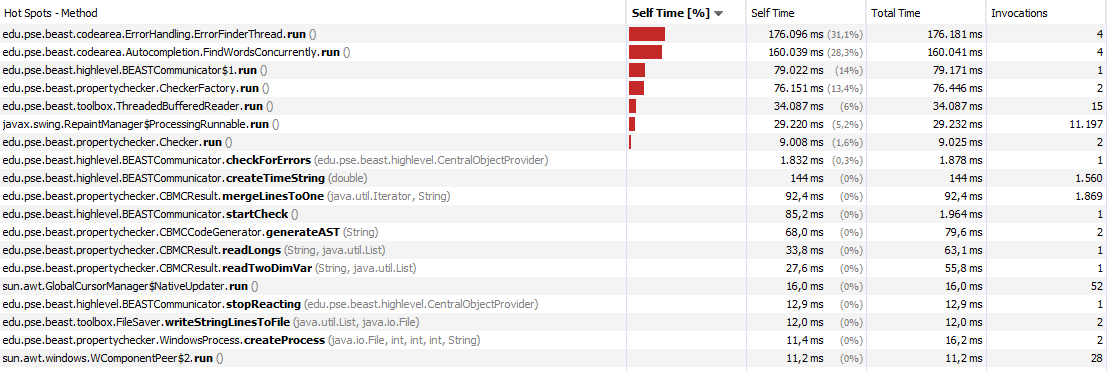
\includegraphics[width=1.0\textwidth,
  height=0.40\textwidth]{images/BEAST_PROCESSORTIME.png} \caption{Der
  Prozentuale Anteil einzelner Methoden an der gesamt benutzen Prozessorzeit}
	\label{fig5}
\end{figure}

\chapter{Fehlerbehebungen}

Nummer problem | Ursache | Lösung


\chapter{Verbesserungen in der Phase}
Neben Fehlerbehebungen haben wir BEAST in dieser Phase auch in einigen Punkten
verbessert:

\begin{itemize}
  \item Im Eigenschafteneditor gibt es nun einen Knopf, welcher eine Erklärung
  über die BooleanExpressionLanguage gibt, mit der der Nutzer hier Befehler
  schreiben kann.
  \item Der Nutzer kann nun als Nach-Eigenschaft angeben, dass die Analyse
  erfolgreich war, wenn ein bestimmter Kandidat gewählt wurde.
\end{itemize}

\chapter{Anhang}

\section{Testprotokolle}
\begin{table}[]
\caption{Testfall 8.1 (Testfälle für die Datenverwaltung)}
\centering
	\begin{tabular}{| p{0.10\linewidth} | p{0.15\linewidth} | p{0.27\linewidth} |
	p{0.15\linewidth} | p{0.09\linewidth} | p{0.09\linewidth} |}
	\hline
	\textbf{Sub-Testfall} &
	\textbf{Abgedeckte Funktionalitäten} &
	\textbf{Beschreibung} &
	\textbf{Ergebnis} & \textbf{Lukas}
	(Windows 10) Version 1.4.22 &
	\textbf{Justin} Lubuntu 16.1 Version 1.4.19
\\
\hline
/T010/ (C-Editor) &
/FS1030/ /FS1100/ /FS1110/ & 
Man gibt ein Wahlverfahren ein. Man wählt in der Toolbar den Button "`Neu"' aus. In einen Dialog gibt man das gewünschte Wahlverfahren und die Anzahl der Sitze ein. In ein Textfeld wird der Name eingegeben. Man drückt auf den Button "`Erstellen"'.
 &
Ein neuer vorgefertigter C-Code erscheint im C-Editor. Ausgegraut sind die Argumente des Wahlverfahrens. &
\Checkmark & \Checkmark
\\
\hline 
/T010/ (Eigenschafteneditor) &
/FM2100/ /FS2150/ &
Man gibt formale Eigenschaften ein. Man wählt in der Toolbar den Button "`Neu"' aus. 
 &
Die Felder für "`Symbolische Variablen"', "`Vorbedingungen"' und "`Nachbedingungen"' leeren sich. In der Titelleiste erscheint der Name "`Eigenschaft 0"'. &
\centering \Checkmark & \Checkmark
\\
\hline 
/T010/ (Eigenschaftenliste) &
/FM3020/ &
Man fügt Eigenschaften zur Liste hinzu. Man wählt in der Toolbar den Button "`Neu"' aus. Die Nachfrage, ob man speichern will, wird verneint.
 &
Die Liste der Eigenschaften leert sich. &
\Checkmark & \Checkmark
\\
\hline 
/T010/ (Parametereditor) &
/FM4050/ &
Man ändert die Parameter. Man wählt in der Toolbar den Button "`Neu"' aus.
 &
Es existiert kein Button für das Neu erstellen. &
X & X
\\
\hline



\end{tabular}
\end{table}
\begin{table}[]
\caption{Testfall 8.1 (Testfälle für die Datenverwaltung)}
\centering
	\begin{tabular}{| p{0.15\linewidth} | p{0.15\linewidth} | p{0.20\linewidth} |
	p{0.15\linewidth} | p{0.1\linewidth} | p{0.1\linewidth} |}
	\hline
	\textbf{Sub-Testfall} &
	\textbf{Abgedeckte Funktionalitäten} &
	\textbf{Beschreibung} &
	\textbf{Ergebnis} & \textbf{Lukas}
	(Windows 10) Version ??? &
	\textbf{Justin} Lubuntu 16.1 Version 1.4.19) 
\\
\hline
/T020/ /T030/ (C-Editor) &
/FM1030/ /FS1100/ /FS1040/ /FS1060/ &
Man gibt ein Wahlverfahren ein. Man wählt in der Toolbar den Button "`Speichern"' aus. In einen Dialog gibt man den gewünschten Speicherort ein. Man drückt auf den Button "`Speichern"'. Man wählt in der Toolbar den Button "`Öffnen"' aus. In einem Dialog wählt man das gespeicherte Wahlverfahren aus.
 &
Das Wahlverfahren wurde gespeichert. Das Laden des Wahlverfahrens schlug fehl. Das Format wurde nicht erkannt. &
\centering . & X
\\
\hline 
/T020/ /T030/ (Eigenschafteneditor) &
/FM2100/ /FS2110/ &
Man gibt formale Eigenschaften ein. Man wählt in der Toolbar den Button "`Speichern"' aus. In einen Dialog gibt man den gewünschten Speicherort ein. Man drückt auf den Button "`Speichern"'. Man wählt in der Toolbar den Button "`Öffnen"' aus. In einem Dialog wählt man die gespeicherten formalen Eigenschaften aus.
 &
Die Eigenschaft wurde gespeichert. Das Laden schlägt fehl. Das Format wurde nicht erkannt. &
\centering . & X
\\
\hline 


\end{tabular}
\end{table}
\begin{table}[]
\caption{Testfall 8.1 (Testfälle für die Datenverwaltung)}
\centering
	\begin{tabular}{| p{0.15\linewidth} | p{0.15\linewidth} | p{0.20\linewidth} |
	p{0.15\linewidth} | p{0.1\linewidth} | p{0.1\linewidth} |}
	\hline
	\textbf{Sub-Testfall} &
	\textbf{Abgedeckte Funktionalitäten} &
	\textbf{Beschreibung} &
	\textbf{Ergebnis} & \textbf{Lukas}
	(Windows 10) Version ??? &
	\textbf{Justin} Lubuntu 16.1 Version 1.4.19) 
\\
\hline 
/T020/ /T030/ (Eigenschaftenliste) &
/FM3060/ /FM3070/ &
Man fügt Eigenschaften zur Liste hinzu. Man wählt in der Toolbar den Button "`Speichern"' aus. In einen Dialog gibt man den gewünschten Speicherort ein. Man drückt auf den Button "`Speichern"'. Man wählt in der Toolbar den Button "`Öffnen"' aus. In einem Dialog wählt man die gespeicherte Eigenschaftenliste aus.
 &
Die Liste der Eigenschaften wurde gespeichert. Die Liste wird wieder geladen. &
\centering . & \Checkmark
\\
\hline 
/T020/ /T030/ (Parametereditor) &
/FM4050/ /FM4060/ &
Man ändert die Parameter. Man wählt in der Toolbar den Button "`Speichern"' aus. In einen Dialog gibt man den gewünschten Speicherort ein. Man drückt auf den Button "`Speichern"'. Man wählt in der Toolbar den Button "`Öffnen"' aus. In einem Dialog wählt man die gespeicherte Eigenschaftenliste aus.
 &
Das Projekt wird gespeichert. Das Projekt kann wieder geladen werden. &
\centering . & \Checkmark
\\ \hline 

\end{tabular}
\end{table}
\begin{table}[]
\caption{Testfall 8.2 (Testfall für Rückgängig machen und Wiederherstellen)}
\centering
	\begin{tabular}{| p{0.15\linewidth} | p{0.15\linewidth} | p{0.20\linewidth} |
	p{0.15\linewidth} | p{0.1\linewidth} | p{0.1\linewidth} |}
	\hline
	\textbf{Sub-Testfall} &
	\textbf{Abgedeckte Funktionalitäten} &
	\textbf{Beschreibung} &
	\textbf{Ergebnis} & \textbf{Lukas}
	(Windows 10) Version 1.4.13 &
	\textbf{Niels} (Linux Mint Cinnamon 3.0.7) Version 1.4.22 
\\
\hline
/T100/ &
/FS1100/ /FS2150/ /F0010/ /F0050/ &
Man startet das Programm ganz normal. Nun gibt man in
jedes Feld, das die "`Rückgängig machen"' Funktionalität unterstützt, einen
kleinen Text ein, und drückt dann, während der Fokus auf dem zu testendem Feld
liegt "`Strg + z"'. &
Der zuletzt eingegebene Buchstabe
oder Textblock (im Falle des Einfügens mit "`Strg + v"') wird gelöscht. &
\Checkmark & \Checkmark 
\\
\hline /T110/& /FS1100/ /FS2150/ /F0010/ /F0050 &
Man startet das Programm ganz normal. Nun gibt man in
jedes Feld, das die "`Rückgängig machen"' Funktionalität unterstützt, einen
kleinen Text ein, und drückt dann, während der Fokus auf dem zu testendem Feld
liegt "`Strg + z"'. Nun drückt man "`Strg + r". &
Der vorher durch das rückgängig machen verschwundene Buchstabe oder Textblock
erscheint wieder. &
\Checkmark 
& \Checkmark  
\\ \hline

\end{tabular}
\end{table}
\begin{table}[]
\caption{Testfall 8.5 (Testfall für das Erstellen einer Eigenschaft im Eigenschafteneditor)}
\centering
	\begin{tabular}{| p{0.15\linewidth} | p{0.15\linewidth} | p{0.20\linewidth} |
	p{0.15\linewidth} | p{0.1\linewidth} | p{0.1\linewidth} |}
	\hline
	\textbf{Sub-Testfall} &
	\textbf{Abgedeckte Funktionalitäten} &
	\textbf{Beschreibung} &
	\textbf{Ergebnis} & \textbf{Lukas}
	(Windows 10) Version 1.4.22 &
	\textbf{Nikolai} Arch Linux (4.10.3-1-ARCH))
\\
\hline
/T410/ &
/FM2040/ /FM2050/ /FM2070/ /FM2071/ /FM2072/ /FM2073/ /FM2080/ /FM2100/ /FM2120/&
Man startet das Programm ganz normal. Nun gibt man im Eigenschafteneditor in den Vorbedingungen 'VOTES1 == VOTES2;', und in den Nachbedingungen 'ELECT1 != ELECT2;' ein. Durch auswählen von "Statische Fehlersuche" testet man die Eigenschaft auf Korrektheit und kann diese anschließend mit dem entsprechenden Menüpunkt oder Toolbar-Button speichern. &
Es wird 'Fehler: 0' im Fehlerfenster angezeigt und die Eigenschaft hat sich ohne Fehlermeldung speichern lassen. &
\Checkmark & \Checkmark
\\
\hline

\end{tabular}
\end{table}
\begin{table}[]
\caption{Testfall 8.6 (Testfälle für die Eigenschaftenliste)}
\centering
	\begin{tabular}{| p{0.10\linewidth} | p{0.15\linewidth} | p{0.27\linewidth} |
	p{0.15\linewidth} | p{0.09\linewidth} | p{0.09\linewidth} |}
	\hline
	\textbf{Sub-Testfall} &
	\textbf{Abgedeckte Funktionalitäten} &
	\textbf{Beschreibung} &
	\textbf{Ergebnis} & \textbf{Lukas}
	(Windows 10) Version 1.4.22 &
	\textbf{Justin} Lubuntu 16.1 Version 1.4.19) 
\\
\hline
/T510/ &
/FM0010/ /FM0020/ /FM0030/ /FM0031/ &
Man gibt ein einfaches Wahlverfahren ein, das eine gewählte Person zurückgibt. Man erstellt eine erste Eigenschaft, die erfüllt ist, und eine zweite Eigenschaft, die nicht erfüllt ist. Man wählt im Parametereditor den Start der Analyse in der Toolbar aus.
 &
Die erste Eigenschaft erscheint grün. Die zweite Eigenschaft erscheint rot. Beim Klick auf das Augensymbol der zweiten Eigenschaft öffnet sich ein Fenster mit einem Gegenbeispiel. &
\Checkmark & \Checkmark
\\
\hline 
/T520/ &
/FM3010/ /FM3050/ &
Man fügt der Eigenschaftenliste eine Eigenschaft hinzu, indem man auf den Button mit dem Pluszeichen und der Beschriftung "`Neu"' drückt. Die Checkbox mit der Beschriftung "`Analyse"' klickt man an. Man wählt im Parametereditor den Start der Analyse in der Toolbar aus.
 &
Die Eigenschaft erscheint grün. Die Eigenschaft wurde von CBMC überprüft. &
\Checkmark & \Checkmark
\\
\hline 
/T530/ &
/FM3010/ FM3020/ &
Man drückt auf den Button mit dem Pluszeichen und der Beschriftung "`Neu"'. 
 &
Eine neue Eigenschaft mit dem Name "`Eigenschaft 0"' erscheint in der Liste. &
\Checkmark & \Checkmark
\\
\hline



\end{tabular}
\end{table}

\end{document}